%%% fs-state-consistency - Fault tolerance

\label {fs-consistency-section}

To fill the gap between the determinism and exactly once we need to design state snapshotting and recovery protocols. In this section, we describe protocols for exactly once enforcement on top of drifting state model introduced in the previous section. While we exploit some properties of this model, proposed protocols can be easily generalized to any deterministic stream processing engine.

% In this section, we outline the implementation details of \\ 
% \FlameStream\ - an open-source prototype implementation of the drifting state model. Firstly, we describe the architecture of our prototype. Then, we demonstrate how exactly nullification tracking and barrier flushing mechanisms work. Finally, the details of snapshotting and failure recovery protocols are shown. 

% \subsection{Meta-information structure}

% In~\FlameStream\ the meta-information is a tuple of a {\it global time}, a {\it trace}, {\it child ids} and a {\it tombstone flag}.

% \[Meta := (GlobalTime, ChildIds[\:], Trace, IsTombstone)\]

% Global time is assigned to each input data item $a$ when it enters the system. It is a logical time and identifier of data producer. The identifier of a data producer is needed to prevent collisions. Global time of a derivative item is a maximal global time among input elements that affect it. This property is preserved in grouping operation and guarantees that if a data flow element $x$ has global time $GT$ and an input element that is defined by global time $GT$ has been already nullified, then all input elements that affect $x$ have been nullified as well. It allows the system to use global time as an indicator of $Cl^{-1}(D)$. It is worth to note that we do not rely on any clock synchronization between nodes. The only implication of the clock skew is the system degradation regarding latency: 1 ms of the fronts clock difference appends 1 ms to minimal latency.

% Map operation is able to generate multiple items from one, and {\em child ids} define an order on them. {\it ChildIds} is an array of child ids, that corresponds to all visited map operations.

% If tombstones have been generated, multiple items with the same global time and child ids can exist in the stream. To differentiate them without the comparison of a payload, there is a {\it Trace} value stored in the meta-information. The trace is a xor of all physical operations' ids (random 64-bit identifier) visited by item so far. Invalid item and the corresponding tombstone go along the same path because they have the same payload and the balancing functions are deterministic. Therefore, item and the corresponding tombstone can be revealed via trace matching. 

% Therefore, on the one hand, meta-information defines a total order on data flow elements (meta is compared lexicographically). On the other hand, it provides additional information about $Cl^{-1}(D)$ and tombstones.

\subsection{Snapshotting}

As it is demonstrated in section~\ref{fs-formalism}, in a deterministic system, state snapshotting and output delivery can be unsynchronized if the system includes in the snapshot last released element as well as system state. The problem here is a need to save at the time $\tau$ snapshot for state $S_{\tau-n}$ for some $n$.

The only stateful operation in the drifting state model is grouping. Hence, there is only a need to save grouping's state in order to take the complete state snapshot. Grouping's state in practice are lists of data items sorted by meta-information. If all input elements $[a_{0}...a_{\tau-n}]$ have been nullified, then state $S_{\tau-n}$ can be snapshotted. Therefore, to take a snapshot at time $\tau$, there is a need to determine maximal $\tau-n$ such that all input elements $[a_{0}...a_{\tau-n}]$ have been nullified. After that, we can just save elements from grouping state lists, which are affected only by these elements. These elements can be determined using meta-information because it contains information about $Cl^{-1}(D)$.

The fact that the only state in the drifting state model has a simple structure of lists sorted by meta-information allows us to take snapshots that contain {\em the past} state. The property of determinism guarantees that such state snapshot together with the last released element is enough to make snapshotting mechanism consistent. The exact protocols, which are used for snapshotting are detailed in the next section.  

\subsubsection{Last output element snapshotting}

As we demonstrated in section~\ref{fs-formalism} if consistent state snapshotting is extended by the snapshotting of the last output element, then a system is able to provide exactly once without synchronization between state snapshotting and output elements releasing. 

Minimal time notifications are sent by the acker with monotonically increasing global times. Barrier receives these notifications and releases output items with monotonically increasing global times as well. Hence, the barrier can filter out any items with a global time less than or equal to the global time of the last released item $GT_{last}$ in order to preserve exactly once. To implement this mechanism, there is a need to atomically output items and update $GT_{last}$. To solve this problem, we require the following output protocol with data consumer: 

\begin{itemize}
    \item When minimal time notification is received, barrier send output bundle to the data consumer. This bundle contains all corresponding output items and $GT_{last}$. The consumer must acknowledge that it received the bundle
    \item Barrier does not send new output bundle until the previous one is not acknowledged
    \item Consumer must return last received bundle on barrier's request 
\end{itemize}

This protocol guarantees that $GT_{last}$ and released items are always consistent with each other. It implies that the barrier can request the last released bundle and fetch $GT_{last}$ after recovery to avoid duplicates and preserve exactly-once semantics.

Thus, on the one hand, we delegate the part of the basic functionality to data consumers. On the other hand, the requirement on data consumer is not so strong and can be naturally satisfied by real-world consumers (HDFS, Kafka, databases, etc.). 

% \subsection{Input replay}

\subsubsection{State snapshotting and input replay}

Input replay functionality is commonly used to restore computational process after a failure in stream processing systems~\cite{Carbone:2017:SMA:3137765.3137777, Akidau:2013:MFS:2536222.2536229, apache:storm}. The key idea here is that in case of failure, previously released input data can be retrieved again. Usually, replay is started not from the beginning, but from a certain point. Like other stream processing solutions, our system requires from producers an ability to replay input data. The only difference is that the initial point of replay is defined in terms of global time. Practically, the role of global times can be played by any monotonically increasing sequence, e.g., offsets in Apache Kafka~\cite{kreps2011kafka} or the values of a logical clock. Therefore, this requirement is not a strong limitation for real-life deployments.

In order to inform data producers that some input data will never be used further, a system must take state snapshots. Because of the fact that in~\FlameStream\ there is no need for synchronization between state snapshotting and elements releasing mechanisms, the global time for taking snapshot can be periodically chosen. It is convenient to piggyback on minimal time notifications for triggering state saving. Let $GT_{min}$ be the last received minimal time within the stream. Grouping's buckets in practice are lists sorted by global time. Because of the guarantees provided by minimal time notifications, these lists cannot be modified at any position before the item that corresponds to $GT_{min}$, the immutable prefix and mutable suffix of grouping bucket are shown at Figure~\ref{immutable}. At the same time, because of the grouping semantics, state that is reached after consuming all data items with global times in range $[0..GT_{min})$ is just a window-sized sublist that is located in the immutable part of the bucket, the example is shown in figure~\ref{substate}. Thereby, state snapshotting of different operations can be done asynchronously with each other and with the computational process of the current operation. 

\begin{figure}[htbp]
  \centering
  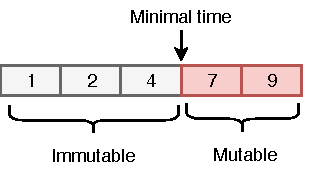
\includegraphics[width=.3\textwidth]{pics/immutable}
  \caption{Grouping bucket won't be modified up to element that corresponds to current minimal time}
  \label {immutable}
\end{figure}

\begin{figure}[htbp]
  \centering
  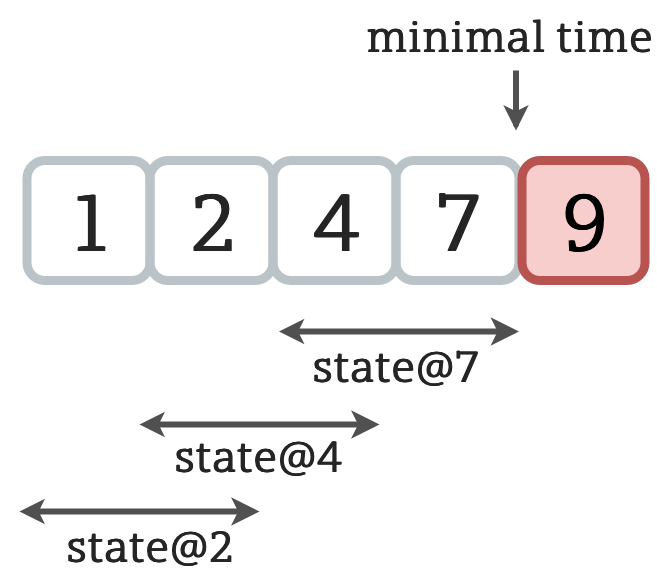
\includegraphics[width=.3\textwidth]{pics/substate}
  \caption{Grouping buckets with window = 2. Window-sized sublists are grouping states at past global times}
  \label {substate}
\end{figure}

Considering the properties mentioned above, the protocol of state snapshotting is the following:

\begin{itemize}
    \item On minimal time event, acker sends a request for the new snapshot along with minimal time notification
    \item When grouping operation receives the request, it asynchronously saves the state and sends back the acceptance message. The local state can be cleared after saving
    \item When barrier receives the request, it waits until producer acknowledges all in-flight bundles, and then sends back the acceptance message to the acker
    \item When acker receives all acceptance messages, it saves the global time of the snapshot to cluster state manager (ZooKeeper) 
\end{itemize}

This protocol is a variation of 2PC and is shown in Algorithm~\ref{state-snapshoting}.

\begin{algorithm}
\caption{State Snapshotting}
\label{state-snapshoting}
  \begin{algorithmic}
    \Process {Acker}
      \State $vertices \gets$ all physical groupings and barrier instances
      \State $snapshotted \gets \varnothing$
      \State $ongoingSnapshot \gets nil$
      \State
      \Event{$\langle MinTime, t \rangle$}
        \If {$ongoingSnapshot = nil$} \Comment{There is no unfinished snapshot}
          \For{{\bf all $v$} $\in vertices$}
            \State \Call{Send}{$v, \langle MinTime_{snap}, t\rangle$}
          \EndFor
          \State $ongoingSnapshot \gets t$
        \EndIf
      \EndEvent
      \Event{$\langle Snapshotted, v\rangle$}
        \State $snapshotted \gets snapshotted \cup v$
        \If {$snapshotted = vertices$}
          \State \Call{Save}{$ongoingSnapshot$} \Comment{Save time to cluster state manager}
          \State $snapshotted \gets \varnothing$
          \State $ongoingSnapshot = nil$
        \EndIf
      \EndEvent
    \EndProcess

    \Process {Grouping}
      \State $bucket[]$ \Comment{List of data items ordered by time}
      \State
      \Event{$\langle MinTime_{snap}, t\rangle$}
        \State \Call{Save}{t, bucket[0, t]} \Comment{Save substate to persistent storage}
        \State \Call{ClearRange}{bucket, 0, t}
        \State \Call{Send}{$acker, \langle Snapshotted, self\rangle$}
      \EndEvent
    \EndProcess

    \Process {Barrier}
      \State $lastAcknowledgedTime \gets -\infty$ \Comment{Time of the last acknowledged bundle by consumer}
      \State $postponedSnapshotTime \gets \infty$
      \State
      \Event{$\langle MinTime_{snap}, t\rangle$}
        \If{$lastAcknowledgedTime \geq t$}
          \State \Call{Send}{$acker, \langle Snapshotted, self\rangle$}
        \Else
          \State $postponedSnapshotTime \gets t$
        \EndIf
      \EndEvent
      \Event{$\langle Ack, t\rangle$}
        \State $lastAcknowledgedTime \gets t$
        \If {$postponedSnapshotTime < lastAcknowledgedTime$}
          \State \Call{Send}{$acker, \langle Snapshotted, self\rangle$}
          \State $postponedSnapshotTime \gets \infty$
        \EndIf
      \EndEvent
    \EndProcess
  \end{algorithmic}
\end{algorithm}

Acker can send requests for the new snapshot not for each minimal time event, e.g., it can skip request if the elapsed time since the last snapshot is less than some threshold. Parameters that influence the frequency of snapshots are in the user's scope.

It is worth to note that any persistent key-value storage can be used as a storage for the state. Hash unit of the corresponding grouping operation concatenated with received minimal time can be used as a key. Waiting until barrier sends out all in-flight bundles is the only dependency between state snapshotting and barrier flushing mechanisms, that does not practically influence end-to-end processing latency. 

This protocol satisfies the following properties regarding the global time $GT$ that is written to cluster state manager:
\begin{enumerate}
    \item All stateful operations can restore the state that is reached after consuming all data items with global times in range $[0..GT)$ 
    \item All bundles that contain items with global times in range $[0..GT)$ have been already acknowledged by data consumer 
\end{enumerate}

Hence, this global time can be used as a resuming point after recovery without loss of consistency.

It is worth to note that the proposed protocol is similar to the state snapshotting protocol used in Flink~\cite{Carbone:2017:SMA:3137765.3137777}. The key difference is that in our method, output releasing agents (barriers) do not take part in a distributed transaction (variation of 2PC), due to drifting state model properties shown in section~\ref{fs-model-section}. This difference determines the significant latency decrease that is demonstrated further.

\subsection{Failure detection and recovery}

Typically, distributed systems take into consideration the following types of failures:
\begin{itemize}
    \item Packet loss
    \item Node failure
    \item Network partitioning
\end{itemize}

Network partitioning is the special case of failure because in this case computations cannot be restarted. We believe that in this case, stream processing does not make sense. To the best of our knowledge, there are no open-source stream processing systems that tolerate network partitioning.

As it was described above, acker traces data items using the table of XORs grouped by global time. Therefore, packet loss can be determined by the acker because the corresponding value in acker's table will not be nullified. Node failure can also be observed by the acker through periodical heartbeats. 

In case of packet loss or node failure, acker restarts the computations from the last successful checkpoint. The failure of the acker itself can be detected by the cluster state manager, that triggers the same restart protocol. Restart protocol includes the following steps:

\begin{itemize}
    \item Acker reads the global time of the last snapshot from a cluster state manager. After that, it broadcasts this global time to all grouping operations
    \item Grouping operations fetch their states from state storage using the corresponding hash unit and received global time as a key. After that, grouping operations send an acknowledgment that they are ready for processing to the acker 
    \item Barriers request the last released bundle from data consumers and send acknowledgments that they are ready for processing to the acker
    \item When acker receives all acknowledgments from groupings and barriers, it requests data producer to replay starting from the global time of the last snapshot  
\end{itemize}

Proposed protocol guarantees the following properties that allow preserving exactly once:

\begin{itemize}
    \item Processing does not restart until all grouping operations obtain consistent states. The consistency of these states is guaranteed by the state snapshotting protocol
    \item Duplicates are not produced because, at the moment when processing is restarted, it is ensured that barrier has obtained the last released global time and is able to filter out extra items
    \item The last released global time cannot be less than the global time of the last snapshot. Therefore, data cannot be lost. This property is guaranteed in conjunction with the state snapshotting protocol
\end{itemize}